% Created 2024-04-02 Τρι 13:35
% Intended LaTeX compiler: pdflatex
\documentclass[11pt]{article}
\usepackage[utf8]{inputenc}
\usepackage[T1]{fontenc}
\usepackage{graphicx}
\usepackage{longtable}
\usepackage{wrapfig}
\usepackage{rotating}
\usepackage[normalem]{ulem}
\usepackage{amsmath}
\usepackage{amssymb}
\usepackage{capt-of}
\usepackage{hyperref}
\usepackage{booktabs}
\usepackage{import}
\usepackage[LGR, T1]{fontenc}
\usepackage[greek, english, american]{babel}
\usepackage{alphabeta}
\usepackage{esint}
\usepackage{mathtools}
\usepackage{esdiff}
\usepackage{makeidx}
\usepackage{glossaries}
\usepackage{newfloat}
\usepackage{minted}
\usepackage[a4paper, margin=3cm]{geometry}
\usepackage{chemfig}
\usepackage{svg}
\author{Vidianos Giannitsis}
\date{\today}
\title{Αποτελέσματα Αναερόβιας Χώνευσης σε BMPs}
\hypersetup{
 pdfauthor={Vidianos Giannitsis},
 pdftitle={Αποτελέσματα Αναερόβιας Χώνευσης σε BMPs},
 pdfkeywords={},
 pdfsubject={},
 pdfcreator={Emacs 29.3 (Org mode 9.6.15)}, 
 pdflang={English}}
\makeatletter
\newcommand{\citeprocitem}[2]{\hyper@linkstart{cite}{citeproc_bib_item_#1}#2\hyper@linkend}
\makeatother

\usepackage[notquote]{hanging}
\begin{document}

\maketitle
\tableofcontents

Σκοπός του αρχείου αυτού είναι η ανάλυση όλων των αποτελεσμάτων των διάφορων πειραμάτων αναερόβιας χώνευσης στην διάταξη για την εύρεση του biomethane potential. Θα αναλυθούν 3 βασικά πειράματα. Το πρώτο είναι η κινητική παραγωγής μεθανίου από οξικό οξύ, ενώ μετά θα αναλυθούν δύο πειράματα παραγωγής μεθανίου από το υδρόλυμα των αποβλήτων τροφών που παράχθηκε στο προηγούμενο στάδιο. Το αρχείο \url{./hplc\_analysis\_notebook.org} περιέχει τα αποτελέσματα των σχετικών πειραμάτων και αναφέρει τα πλεονεκτήματα και μειονεκτήματα τους.

\section{Dependencies}
\label{sec:org9916056}
Στο αρχείο αυτό θα οριστούν κάποια functions για να διευκολυνθεί η ανάλυση των BMPs, τα οποία θα είναι generic και μετά θα υπάρχουν κάποια specific code blocks για την εφαρμογή σε κάθε πείραμα. Πριν ξεκινήσουμε, κάνουμε activate το DrWatson project για reproducibility. Επίσης κάνουμε load το Dates.jl που θα χρειαστεί παρακάτω, καθώς και τα CSV.jl και DataFrames.jl που είναι πάντα χρήσιμα σε tabular data. Ακόμη, παρακάτω θα χρειαστούν τα LsqFit.jl για την προσαρμογή του μοντέλου Gompertz, StatsBase για υπολογισμό μέσων και Plots.jl για plotting. Το code block αυτό δεν κάνει tangle πουθενά καθώς είναι κομμάτι του generic code που θα χρησιμοποιηθεί σε πολλά σημεία.

\textbf{deps}
\begin{minted}[breaklines=true,breakanywhere=true]{julia}

using DrWatson
@quickactivate "Masters_Thesis"

using Dates
using CSV, DataFrames
using LsqFit
using StatsBase
using Plots

\end{minted}

\section{Acetate Experiment data reading}
\label{sec:org3238a80}
Τα δεδομένα της αναερόβιας χώνευσης είναι φωτογραφίες των προχωίδων της διάταξης. ΕΞετάζοντας πόσο έχει μεταβληθεί η στάθμη τους, μπορούμε να υπολογίσουμε τον παραγόμενο όγκο μεθανίου. Αλλά πρώτα, πρέπει να ξέρουμε σε τι χρόνους έγιναν sampled τα δείγματα. Όλες οι φωτογραφίες έχουν ένα timestamp το οποίο μας βοηθάει να τα διακρίνουμε. Μπορούμε να αναλύσουμε αυτά ώστε να πάρουμε τις στιγμές που βγήκαν οι φωτογραφίες. Αρχικά, παίρνουμε όλα τα filenames με \texttt{ls}. Θα χρησιμοποιήσουμε τα flags -m και -Q για να πάρουμε comma separated output και το κάθε string να έχει double quotes.

\textbf{ls\textsubscript{output}\textsubscript{acetate}}
\begin{minted}[breaklines=true,breakanywhere=true]{sh}
ls -mQ ../bmp_pictures/Acet_kinetics_screenshots/
\end{minted}

\begin{verbatim}
"bandicam 2024-03-27 18-45-55-857.jpg", "bandicam 2024-03-27 18-46-57-161.jpg",
"bandicam 2024-03-27 18-48-57-160.jpg", "bandicam 2024-03-27 18-50-57-170.jpg",
"bandicam 2024-03-27 18-52-57-164.jpg", "bandicam 2024-03-27 18-54-57-162.jpg",
"bandicam 2024-03-27 18-56-57-167.jpg", "bandicam 2024-03-27 18-58-57-165.jpg",
"bandicam 2024-03-27 19-00-57-170.jpg", "bandicam 2024-03-27 19-02-57-179.jpg",
"bandicam 2024-03-27 19-04-57-173.jpg", "bandicam 2024-03-27 19-06-57-182.jpg",
"bandicam 2024-03-27 19-08-57-185.jpg", "bandicam 2024-03-27 19-10-57-184.jpg",
"bandicam 2024-03-27 19-12-57-189.jpg", "bandicam 2024-03-27 19-14-57-187.jpg",
"bandicam 2024-03-27 19-15-06-279.jpg", "bandicam 2024-03-27 19-19-06-273.jpg",
"bandicam 2024-03-27 19-21-06-276.jpg", "bandicam 2024-03-27 19-23-06-285.jpg",
"bandicam 2024-03-27 19-25-06-290.jpg", "bandicam 2024-03-27 19-27-06-301.jpg",
"bandicam 2024-03-27 19-29-06-303.jpg", "bandicam 2024-03-27 19-31-06-301.jpg",
"bandicam 2024-03-27 19-33-06-297.jpg", "bandicam 2024-03-27 19-35-06-305.jpg",
"bandicam 2024-03-27 19-37-06-299.jpg", "bandicam 2024-03-27 19-39-06-297.jpg",
"bandicam 2024-03-27 19-41-06-307.jpg", "bandicam 2024-03-27 19-43-06-299.jpg",
"bandicam 2024-03-27 19-45-06-298.jpg", "bandicam 2024-03-27 19-47-06-304.jpg",
"bandicam 2024-03-27 19-48-50-591.jpg", "bandicam 2024-03-29 12-23-36-175.jpg",
"bandicam 2024-03-29 12-23-50-142.jpg", "bandicam 2024-03-29 12-24-50-161.jpg",
"bandicam 2024-03-29 12-25-50-156.jpg", "bandicam 2024-03-29 12-26-50-168.jpg",
"bandicam 2024-03-29 12-27-26-514.jpg", "bandicam 2024-03-29 12-28-26-502.jpg",
"bandicam 2024-03-29 12-29-26-497.jpg", "bandicam 2024-03-29 12-29-39-894.jpg",
"bandicam 2024-03-29 12-30-39-902.jpg", "bandicam 2024-03-29 12-31-39-897.jpg",
"bandicam 2024-03-29 12-32-05-844.jpg", "bandicam 2024-03-29 12-33-05-843.jpg",
"bandicam 2024-03-29 12-34-05-832.jpg", "bandicam 2024-03-29 12-35-05-836.jpg",
"bandicam 2024-03-29 12-36-05-835.jpg", "bandicam 2024-03-29 12-37-05-858.jpg",
"bandicam 2024-03-29 12-38-06-101.jpg", "bandicam 2024-03-29 12-38-47-045.jpg",
"bandicam 2024-03-29 12-39-47-039.jpg", "bandicam 2024-03-29 12-40-47-050.jpg",
"bandicam 2024-03-29 12-41-47-047.jpg", "bandicam 2024-03-29 12-42-47-057.jpg",
"bandicam 2024-03-29 12-43-42-169.jpg", "bandicam 2024-03-29 12-44-41-398.jpg"
\end{verbatim}

Αρχικά, κάνουμε load τα dependencies στο script στο οποίο θα γίνει η ανάλυση του πειράματος αυτού.

\begin{minted}[breaklines=true,breakanywhere=true]{julia}

<<deps>>

\end{minted}

Έπειτα, ξεκινάμε την ανάλυση αποθηκεύοντας τα file names σε ένα vector της Julia κάνοντας copy τα shell results. Αυτό το vector θα γίνεται loaded σε όλα τα code blocks, για να είναι το κάθε ένα reproducible από μόνο του. Έτσι, στο τελικό script θα υπάρχουν πολλές επαναλήψεις.

\textbf{date\textsubscript{saving}\textsubscript{acetate}}
\begin{minted}[breaklines=true,breakanywhere=true]{julia}

file_vec = ["bandicam 2024-03-27 18-45-55-857.jpg", "bandicam 2024-03-27 18-46-57-161.jpg",
"bandicam 2024-03-27 18-48-57-160.jpg", "bandicam 2024-03-27 18-50-57-170.jpg",
"bandicam 2024-03-27 18-52-57-164.jpg", "bandicam 2024-03-27 18-54-57-162.jpg",
"bandicam 2024-03-27 18-56-57-167.jpg", "bandicam 2024-03-27 18-58-57-165.jpg",
"bandicam 2024-03-27 19-00-57-170.jpg", "bandicam 2024-03-27 19-02-57-179.jpg",
"bandicam 2024-03-27 19-04-57-173.jpg", "bandicam 2024-03-27 19-06-57-182.jpg",
"bandicam 2024-03-27 19-08-57-185.jpg", "bandicam 2024-03-27 19-10-57-184.jpg",
"bandicam 2024-03-27 19-12-57-189.jpg", "bandicam 2024-03-27 19-14-57-187.jpg",
"bandicam 2024-03-27 19-15-06-279.jpg", "bandicam 2024-03-27 19-19-06-273.jpg",
"bandicam 2024-03-27 19-21-06-276.jpg", "bandicam 2024-03-27 19-23-06-285.jpg",
"bandicam 2024-03-27 19-25-06-290.jpg", "bandicam 2024-03-27 19-27-06-301.jpg",
"bandicam 2024-03-27 19-29-06-303.jpg", "bandicam 2024-03-27 19-31-06-301.jpg",
"bandicam 2024-03-27 19-33-06-297.jpg", "bandicam 2024-03-27 19-35-06-305.jpg",
"bandicam 2024-03-27 19-37-06-299.jpg", "bandicam 2024-03-27 19-39-06-297.jpg",
"bandicam 2024-03-27 19-41-06-307.jpg", "bandicam 2024-03-27 19-43-06-299.jpg",
"bandicam 2024-03-27 19-45-06-298.jpg", "bandicam 2024-03-27 19-47-06-304.jpg",
"bandicam 2024-03-27 19-48-50-591.jpg", "bandicam 2024-03-29 12-23-36-175.jpg",
"bandicam 2024-03-29 12-23-50-142.jpg", "bandicam 2024-03-29 12-24-50-161.jpg",
"bandicam 2024-03-29 12-25-50-156.jpg", "bandicam 2024-03-29 12-26-50-168.jpg",
"bandicam 2024-03-29 12-27-26-514.jpg", "bandicam 2024-03-29 12-28-26-502.jpg",
"bandicam 2024-03-29 12-29-26-497.jpg", "bandicam 2024-03-29 12-29-39-894.jpg",
"bandicam 2024-03-29 12-30-39-902.jpg", "bandicam 2024-03-29 12-31-39-897.jpg",
"bandicam 2024-03-29 12-32-05-844.jpg", "bandicam 2024-03-29 12-33-05-843.jpg",
"bandicam 2024-03-29 12-34-05-832.jpg", "bandicam 2024-03-29 12-35-05-836.jpg",
"bandicam 2024-03-29 12-36-05-835.jpg", "bandicam 2024-03-29 12-37-05-858.jpg",
"bandicam 2024-03-29 12-38-06-101.jpg", "bandicam 2024-03-29 12-38-47-045.jpg",
"bandicam 2024-03-29 12-39-47-039.jpg", "bandicam 2024-03-29 12-40-47-050.jpg",
"bandicam 2024-03-29 12-41-47-047.jpg", "bandicam 2024-03-29 12-42-47-057.jpg",
"bandicam 2024-03-29 12-43-42-169.jpg", "bandicam 2024-03-29 12-44-41-398.jpg"
]

\end{minted}

\section{Data Processing}
\label{sec:org5c75afa}
Έπειτα, μπορούμε να κάνουμε extract τις πληροφορίες που θέλουμε, με το Dates.jl package της Julia. Σε αυτό το code block, δεν θα ορίσουμε το file vector και αυτό θα υποτεθεί defined. Έτσι, δεν μπορούμε να τρέξουμε independently το block αυτό, αλλά μόνο chained σε ένα definition των files, για να μπορεί να τρέξει αντίστοιχα σε κάθε πείραμα. Επίσης, εκτός από να κάνουμε extract τα time stamps, φτιάχνουμε και ένα δεύτερο vector με time stamp dd/mm\textsubscript{HH}:MM το οποίο είναι πιο βολικό στη χρήση για εμένα.

Στη συνέχεια, ορίζουμε άλλη μία μεταβλητή η οποία δεν υπάρχει, η \texttt{inds}. Αυτή είναι τα νούμερα στο date\textsubscript{vec} που αντιστοιχούν σε ένα ορισμένο πείραμα. Παίρνουμε τα time stamps και στην αρχική αλλά και στην formatted μορφή για αυτό το πείραμα και μετά υπολογίζουμε τα time steps και σε δευτερόλεπτα αλλά και σε λεπτά. Η αφαίρεση δύο \texttt{DateTime} objects δίνει αποτέλεσμα σε \texttt{Millisecond}, οπότε ο χρόνος σε δευτερόλεπτα διαιρεί με 1000 \texttt{Millisecond} ενώ σε λεπτά με 60000 \texttt{Millisecond}. Έπειτα, ορίζουμε ένα τρίτο undefined variable το exp\textsubscript{meth}\textsubscript{vol}, το οποίο είναι η παραγωγή μεθανίου μεταξύ των δύο φωτογραφιών, όπως σημειώνεται σε αυτές. Για την κινητική, θέλουμε την αθροιστική παραγωγή μεθανίου, οπότε χρησιμοποιούμε την συνάρτηση \texttt{cumsum}. Τέλος, αποθηκεύουμε όλα αυτά τα δεδομένα σε ένα table του \texttt{Tables.jl} interface, ώστε να μπορούμε να το κάνουμε DataFrame με headers για καλύτερο readability ή να το κάνουμε export σε csv. Για το csv export χρειαζόμαστε ένα file name. Αυτό μπορεί για άλλη μία φορά να μην οριστεί εδώ και να χρησιμοποιηθεί ως variable.

\textbf{bmp\textsubscript{data}\textsubscript{processing}}
\begin{minted}[breaklines=true,breakanywhere=true]{julia}

date_vec = [DateTime(SubString(file_vec[i], 10, 32), "yyyy-mm-dd HH-MM-SS-sss") for i in 1:length(file_vec)]
formatted_date = [Dates.format(date_vec[i], "dd/mm_HH:MM") for i in 1:length(date_vec)]

exp_stamps = date_vec[inds]
exp_formatted = formatted_date[inds]
exp_sec = [(exp_stamps[i] - exp_stamps[1])/Millisecond(1000) for i in 1:(last(inds) - first(inds) + 1)]
exp_min = [(exp_stamps[i] - exp_stamps[1])/Millisecond(60000) for i in 1:(last(inds) - first(inds) + 1)]
exp_cum_meth_vol = cumsum(exp_meth_vol)

exp_data = Tables.table(hcat(exp_formatted, exp_sec, exp_min, exp_meth_vol, exp_cum_meth_vol), header = [:Timestamp, :Seconds, :Minutes, :Methane_Volume, :Cumulative_Methane_Volume])
CSV.write(datadir("exp_pro", exp_name*".csv"), exp_data)
exp_df = DataFrame(exp_data)

\end{minted}

\subsection{Curve Fitting}
\label{sec:orgc834d79}
Επίσης, θέλουμε να κάνουμε fit τα δεδομένα σε κάποιο κινητικό μοντέλο για την διεργασία, κάτι το οποίο θα βοηθήσει στη μοντελοποιήση της. Το μοντέλο Gompertz είναι ένα μοντέλο που χρησιμοποιείται συχνά για kinetic modelling διεργασιών όπως η παραγωγή μεθανίου μέσω αναερόβιας χώνευσης, οπότε θα χρησιμοποιηθεί αυτό. Η εξίσωση που θα πρέπει να προσαρμοστεί είναι η
\[ P(t) = P_{\max } \exp \left( - \exp \left[ \frac{R_{\max }e (λ-t)}{P_{\max }} + 1 \right] \right) \]
όπου P(t) η παραγωγή μεθανίου την στιγμή t, P\textsubscript{max} η μέγιστη ποσότητα μεθανίου που μπορεί να παραχθεί από το υπόστρωμα αυτό, R\textsubscript{max} ο ειδικός ρυθμός παραγωγής μεθανίου, λ το lag time και e η σταθερά Euler. Παρακάτω φαίνεται το fit των δεδομένων στην συνάρτηση αυτή. Αξίζει να αναφερθεί η χρήση της μεταβλητής \texttt{input\_cod} που φαίνεται παρακάτω. Η μεταβλητή αυτή εκφράζει το COD της τροφοδοσίας. Διαιρούμε τον όγκο μεθανίου με αυτήν ώστε το διάγραμμα να εκφράζει ειδικό ρυθμό παραγωγής μεθανίου σε \(\frac{\text{mL CH$_4$}}{\text{g sCOD}}\), το οποίο είναι πιο εύκολα συγκρίσιμο με βιβλιογραφία, σε σχέση με τον όγκο μεθανίου. Επίσης, αξίζει να σημειωθεί η χρήση bounded optimization. Οι παραμέτροι του μοντέλου έχουν νόημα μόνο ως θετικοί αριθμοί. Στα πειράματα με χρήση οξικό ως υπόστρωμα, όπου οι μικροοργανισμοί αντιδρούν ταχύτατα στην αλλαγή του περιβάλλοντος, η προσαρμογή του μοντέλου έδινε αρνητικό lag time. Αυτό προφανώς δεν έχει νόημα και στην πράξη, το συμπέρασμα είναι πως το lag time είναι μηδενικό (σχεδόν ακαριαία αντίδραση των μικροοργανισμών στην προσθήκη οξικού στο σύστημα). Επίσης, αξίζει να αναφερθεί η μεταβλητή \texttt{kinetics}. Σε κάποια πειράματα (πχ τις μετρήσεις παραγωγής μεθανίου χωρίς προσθήκη υποστρώματος που έγινε σε ένα δείγμα) δεν θέλουμε να κάνουμε προσαρμογή με το μοντέλο Gompertz. Αυτή η μεταβλητή είναι στην ουσία ένα toggle off του plot με την κινητική, για όσα πειράματα δεν το χρειάζονται.

\textbf{bmp\textsubscript{curve}\textsubscript{fitting}}
\begin{minted}[breaklines=true,breakanywhere=true]{julia}

gompertz(t, p) = @. p[1]*exp(-exp((((p[2]*exp(1))/p[1])*(p[3] - t)) + 1))
p0 = [300.0, 50.0, 1.0]
lb = [0.0, 0.0, 0.0]
ub = [Inf, Inf, Inf]
specific_meth_vol = exp_cum_meth_vol./input_cod

fit = curve_fit(gompertz, exp_min, specific_meth_vol, p0, lower = lb, upper = ub)
model_params = fit.param
gompertz(t) = gompertz(t, model_params)

model_res = fit.resid
SS_res = sum(model_res.^2)
SS_tot = sum([(specific_meth_vol[i] - mean(specific_meth_vol)).^2 for i in 1:length(specific_meth_vol)])
r_squared = 1 - SS_res/SS_tot

kinetics = true

\end{minted}

\subsection{Plotting}
\label{sec:orgb53eb5c}
Τέλος, έχοντας προσαρμώσει το μοντέλο Gompertz σε κάθε σετ δεδομένων, θέλουμε να φτιάξουμε κάποια διαγράμματα με τα δεδομένα, τα οποία να δείχνουν την παραγόμενη ποσότητα μεθανίου στον χρόνο. Τα πειραματικά δεδομένα θα γίνουν plotted σε scatter plots. Χάριν ευκολίας, μπορούν να γίνουν plotted διαγράμματα και της στιγμιαίας αλλά και της συνολικής παραγωγής μεθανίου και σε άξονα χρόνου είτε λεπτά ή δευτερόλεπτα. Ο παραπάνω κώδικας υπολογίζει το fit του cumulative methane production σε λεπτά, καθώς θεωρείται η πιο χρήσιμη έκφραση, οπότε αυτό θα είναι και το διάγραμμα που έχει fit την καμπύλη. Εδώ θα εκμεταλλευτούμε τα variables που υπολογίζονται παραπάνω καθώς και 2 ακόμη, το \texttt{sample} και το \texttt{source}. Το \texttt{source} είναι ένα απλό variable το οποίο εκφράζει αν η τροφοδοσία ήταν οξικό ή υδρόλυμα για να τα ξεχωρίζουμε πιο εύκολα. Το \texttt{sample} εκφράζει το νούμερο του δείγματος για να είναι πιο εύκολο το naming scheme.

\textbf{bmp\textsubscript{data}\textsubscript{plotting}}
\begin{minted}[breaklines=true,breakanywhere=true]{julia}


bmp_cumulative_scatter_sec = scatter(exp_sec, exp_cum_meth_vol, markersize = 5, legend = false, xlabel = "Time (sec)", ylabel = "Cumulative Methane Volume (mL)", title = "Cumulative Methane Production from "*source*" - "*sample, size = (700, 470))
savefig(bmp_cumulative_scatter_sec, plotsdir("BMPs", source, "cumulative_"*exp_name*"_sec.png"))

bmp_cumulative_scatter_min = scatter(exp_min, exp_cum_meth_vol, markersize = 5, legend = false, xlabel = "Time (min)", ylabel = "Cumulative Methane Volume (mL)", title = "Cumulative Methane Production from "*source*" - "*sample, size = (700, 470))
savefig(bmp_cumulative_scatter_min, plotsdir("BMPs", source, "cumulative_"*exp_name*"_min.png"))

if kinetics
    bmp_specific_methane = scatter(exp_min, specific_meth_vol, markersize = 5, label = "Experimental Data", xlabel = "Time (min)", ylabel = "Cumulative Methane Production (mL/g sCOD)", title = "Methane Production Kinetics from "*source*" - "*sample, size = (700, 470), legend = :bottomright)
    plot!(exp_min, gompertz(exp_min), label = "Gompertz Model with R^2 = "*string(round(r_squared, digits = 3)))
    savefig(bmp_specific_methane, plotsdir("BMPs", source, "methane_kinetics_"*exp_name*".png"))
end

bmp_scatter_sec = scatter(exp_sec, exp_meth_vol, markersize = 5, legend = false, xlabel = "Time (sec)", ylabel = "Methane Volume (mL)", title = "Methane Production from "*source*" - "*sample)
savefig(bmp_scatter_sec, plotsdir("BMPs", source, exp_name*"_sec.png"))

bmp_scatter_min = scatter(exp_min, exp_meth_vol, markersize = 5, legend = false, xlabel = "Time (min)", ylabel = "Methane Volume (mL)", title = "Methane Production from "*source*" - "*sample)
savefig(bmp_scatter_min, plotsdir("BMPs", source, exp_name*"_min.png"))

\end{minted}

\section{Acetate Experiment Processing}
\label{sec:orge0936a8}
Παρακάτω αναφέρονται οι δοκιμές που έγιναν με 100 μL οξικό σε κάθε δείγμα και θα χρησιμοποιηθούν πιθανόν συγκριτικά σε σχέση με τα FW. Μετά από τα code blocks που τρέχουν τον κώδικα θα υπάρχουν και κάποια από τα corresponding αποτελέσματα. Συγκεκριμένα, ο πίνακας με τα κινητικά δεδομένα, το διάγραμμα παραγωγής μεθανίου το οποίο έχει το curve fitting και το διάγραμμα στιγμίαιας παραγωγής μεθανίου. Υπάρχουν και κάποια άλλα χρήσιμα διαγράμματα, τα οποία είναι αποθηκευμένα, αλλά εδώ παρατίθενται κάποια για καλύτερη ανάγνωση του αρχείου.

\subsection{Acetate Test 1}
\label{sec:orgf142137}
Το section αυτό αναφέρεται στη δοκιμή με 100 μL οξικό στο δείγμα (1). Notably, δεν είχε διαρροή στις 27/03, αλλά για κάποιον λόγο, στην επαναδοκιμή στις 29/03 δεν παρήγαγε μεθάνιο (τουλάχιστον στην προχοίδα). Οπότε, θα χρησιμοποιηθεί αυτό της 27/03.

\textbf{acet\textsubscript{test}\textsubscript{1}}
\begin{minted}[breaklines=true,breakanywhere=true]{julia}

### Data Analysis on Sample 1 ###

<<date_saving_acetate>>

inds = 1:12
exp_meth_vol = [0, 12, 5, 3, 1.5, 1.5, 1, 1.5, 1, 0.5, 0.5, 0.5]
exp_name = "acet_test_1"
source = "Acetate"
sample = "Sample 1"
input_cod = 0.1

<<bmp_data_processing>>
<<bmp_curve_fitting>>
model_acet_1 = vcat(sample, model_params, r_squared)
<<bmp_data_plotting>>
\end{minted}

\begin{table}[htbp]
\caption{Κινητικά δεδομένα}
\centering
\begin{tabular}{lrrrr}
Timestamp & Seconds & Minutes & Methane\textsubscript{Volume} & Cumulative\textsubscript{Methane}\textsubscript{Volume}\\[0pt]
\hline
27/03\textsubscript{18}:45 & 0.0 & 0.0 & 0.0 & 0.0\\[0pt]
27/03\textsubscript{18}:46 & 61.304 & 1.02173 & 12.0 & 12.0\\[0pt]
27/03\textsubscript{18}:48 & 181.303 & 3.02172 & 5.0 & 17.0\\[0pt]
27/03\textsubscript{18}:50 & 301.313 & 5.02188 & 3.0 & 20.0\\[0pt]
27/03\textsubscript{18}:52 & 421.307 & 7.02178 & 1.5 & 21.5\\[0pt]
27/03\textsubscript{18}:54 & 541.305 & 9.02175 & 1.5 & 23.0\\[0pt]
27/03\textsubscript{18}:56 & 661.31 & 11.0218 & 1.0 & 24.0\\[0pt]
27/03\textsubscript{18}:58 & 781.308 & 13.0218 & 1.5 & 25.5\\[0pt]
27/03\textsubscript{19}:00 & 901.313 & 15.0219 & 1.0 & 26.5\\[0pt]
27/03\textsubscript{19}:02 & 1021.322 & 17.0220 & 0.5 & 27.0\\[0pt]
27/03\textsubscript{19}:04 & 1141.316 & 19.0219 & 0.5 & 27.5\\[0pt]
27/03\textsubscript{19}:06 & 1261.325 & 21.0220 & 0.5 & 28.0\\[0pt]
\end{tabular}
\end{table}

\begin{center}
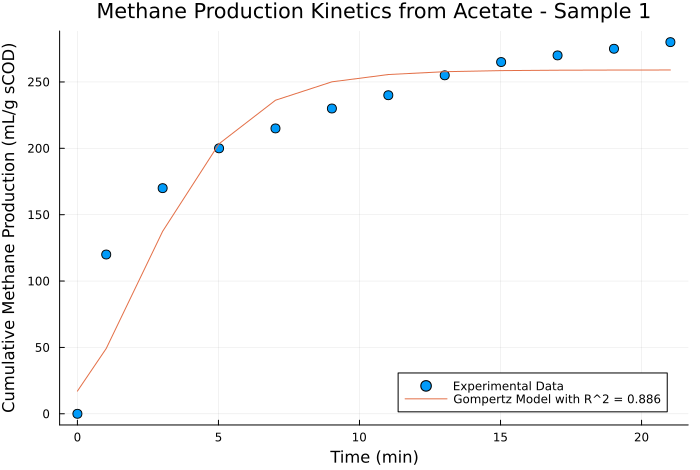
\includegraphics[width=.9\linewidth]{../plots/BMPs/Acetate/methane_kinetics_acet_test_1.png}
\end{center}

\begin{center}
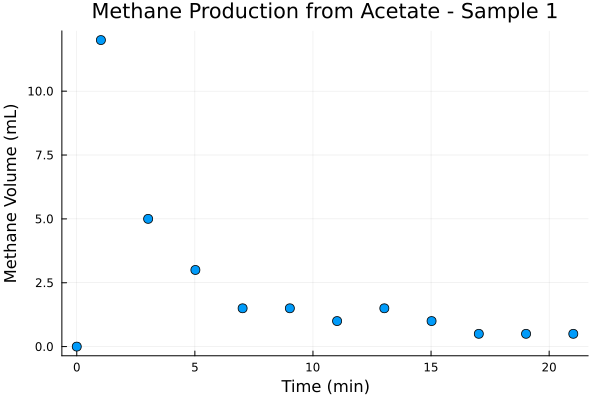
\includegraphics[width=.9\linewidth]{../plots/BMPs/Acetate/acet_test_1_min.png}
\end{center}

\subsection{Acetate Test 0}
\label{sec:orgbfd6eb3}
Το section αυτό αναφέρεται στη δοκιμή με 100 μL οξικό στο δείγμα (0).

\textbf{acet\textsubscript{test}\textsubscript{0}}
\begin{minted}[breaklines=true,breakanywhere=true]{julia}

### Data Analysis on Sample 0 ###

<<date_saving_acetate>>

inds = 34:51
exp_meth_vol = [0, 4, 12, 7.5, 4.5, 2.5, 2.5, 4, 0.5, 2, 2, 1, 1, 1, 1, 1, 0.5, 0.5]
exp_name = "acet_test_0"
source = "Acetate"
sample = "Sample 0"
input_cod = 0.1

<<bmp_data_processing>>
<<bmp_curve_fitting>>
model_acet_0 = vcat(sample, model_params, r_squared)
<<bmp_data_plotting>>
\end{minted}

\begin{table}[htbp]
\caption{Κινητικά δεδομένα}
\centering
\begin{tabular}{lrrrr}
Timestamp & Seconds & Minutes & Methane\textsubscript{Volume} & Cumulative\textsubscript{Methane}\textsubscript{Volume}\\[0pt]
\hline
29/03\textsubscript{12}:23 & 0.0 & 0.0 & 0.0 & 0.0\\[0pt]
29/03\textsubscript{12}:23 & 13.967 & 0.2327 & 4.0 & 4.0\\[0pt]
29/03\textsubscript{12}:24 & 73.986 & 1.2331 & 12.0 & 16.0\\[0pt]
29/03\textsubscript{12}:25 & 133.981 & 2.2330 & 7.5 & 23.5\\[0pt]
29/03\textsubscript{12}:26 & 193.993 & 3.2332 & 4.5 & 28.0\\[0pt]
29/03\textsubscript{12}:27 & 230.339 & 3.8389 & 2.5 & 30.5\\[0pt]
29/03\textsubscript{12}:28 & 290.327 & 4.8388 & 2.5 & 33.0\\[0pt]
29/03\textsubscript{12}:29 & 350.322 & 5.8387 & 4.0 & 37.0\\[0pt]
29/03\textsubscript{12}:29 & 363.719 & 6.0619 & 0.5 & 37.5\\[0pt]
29/03\textsubscript{12}:30 & 423.727 & 7.0621 & 2.0 & 39.5\\[0pt]
29/03\textsubscript{12}:31 & 483.722 & 8.0620 & 2.0 & 41.5\\[0pt]
29/03\textsubscript{12}:32 & 509.669 & 8.4945 & 1.0 & 42.5\\[0pt]
29/03\textsubscript{12}:33 & 569.668 & 9.4945 & 1.0 & 43.5\\[0pt]
29/03\textsubscript{12}:34 & 629.657 & 10.4943 & 1.0 & 44.5\\[0pt]
29/03\textsubscript{12}:35 & 689.661 & 11.4943 & 1.0 & 45.5\\[0pt]
29/03\textsubscript{12}:36 & 749.66 & 12.4943 & 1.0 & 46.5\\[0pt]
29/03\textsubscript{12}:37 & 809.683 & 13.4947 & 0.5 & 47.0\\[0pt]
29/03\textsubscript{12}:38 & 869.926 & 14.4987 & 0.5 & 47.5\\[0pt]
\end{tabular}
\end{table}

\begin{center}
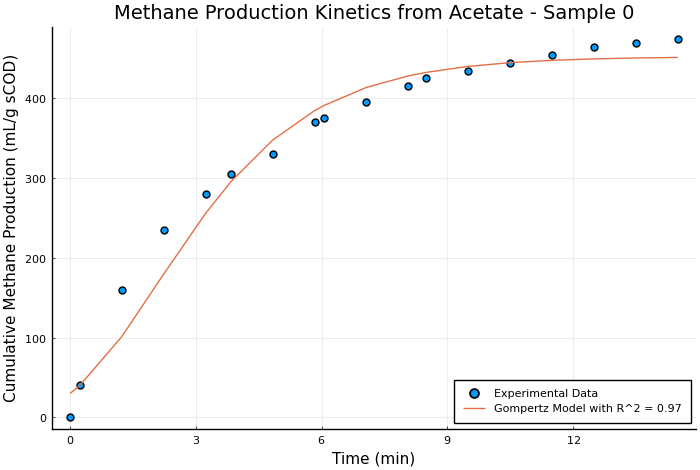
\includegraphics[width=.9\linewidth]{../plots/BMPs/Acetate/methane_kinetics_acet_test_0.png}
\end{center}

\begin{center}
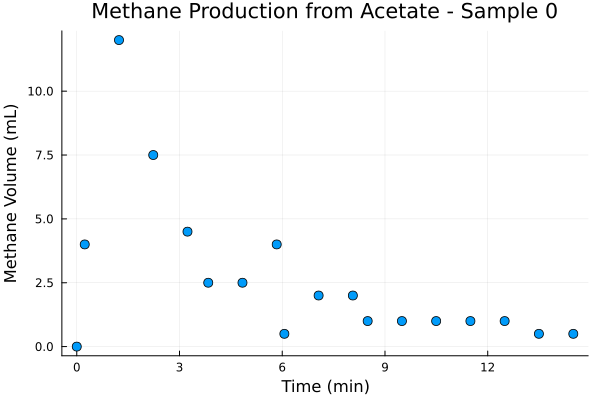
\includegraphics[width=.9\linewidth]{../plots/BMPs/Acetate/acet_test_0_min.png}
\end{center}


\subsection{Acetate Test Ac}
\label{sec:orge262c4d}
Το section αυτό αναφέρεται στη δοκιμή με 100 μL οξικό στο δείγμα (Ac). Το δείγμα αυτό είναι αυτό που δεν θα τροφοδοτηθεί με κάποιο από τα υδρολύματα των FW αλλά θα χρησιμοποιηθεί ως blank, οπότε είναι labelled ως Acetate. Για αυτό, αξίζει να αναφερθεί πως την πρώτη πειραματική ημέρα (27/03), παρήγαγε αέριο χωρίς να τροφοδοτηθεί με κάποιο υπόστρωμα. Η κινητική αυτής της παραγωγής (η οποία δεν ξέρουμε σε τι ευθύνεται) θα αναλυθεί παρακάτω. Βέβαια, μόλις τροφοδοτήθηκε με οξικό και η παραγωγή του τελείωσε, σταμάτησε και εκείνη η παραγωγή.

\textbf{acet\textsubscript{test}\textsubscript{ac}}
\begin{minted}[breaklines=true,breakanywhere=true]{julia}

### Data Analysis on Sample Ac ###

<<date_saving_acetate>>

inds = 38:56
exp_meth_vol = [0, 6.5, 5, 3, 0.5, 1.5, 1.5, 0.5, 1, 0.5, 0.5, 0.3, 0.2, 0.2, 0.1, 0.05, 0.05, 0.05, 0.05]
exp_name = "acet_test_ac"
source = "Acetate"
sample = "Sample Ac"
input_cod = 0.1

<<bmp_data_processing>>
<<bmp_curve_fitting>>
model_acet_ac = vcat(sample, model_params, r_squared)
<<bmp_data_plotting>>
\end{minted}

\begin{table}[htbp]
\caption{Κινητικά δεδομένα}
\centering
\begin{tabular}{lrrrr}
Timestamp & Seconds & Minutes & Methane\textsubscript{Volume} & Cumulative\textsubscript{Methane}\textsubscript{Volume}\\[0pt]
\hline
29/03\textsubscript{12}:26 & 0.0 & 0.0 & 0.0 & 0.0\\[0pt]
29/03\textsubscript{12}:27 & 36.346 & 0.6058 & 6.5 & 6.5\\[0pt]
29/03\textsubscript{12}:28 & 96.334 & 1.6055 & 5.0 & 11.5\\[0pt]
29/03\textsubscript{12}:29 & 156.329 & 2.6055 & 3.0 & 14.5\\[0pt]
29/03\textsubscript{12}:29 & 169.726 & 2.8288 & 0.5 & 15.0\\[0pt]
29/03\textsubscript{12}:30 & 229.734 & 3.8289 & 1.5 & 16.5\\[0pt]
29/03\textsubscript{12}:31 & 289.729 & 4.8288 & 1.5 & 18.0\\[0pt]
29/03\textsubscript{12}:32 & 315.676 & 5.2613 & 0.5 & 18.5\\[0pt]
29/03\textsubscript{12}:33 & 375.675 & 6.2612 & 1.0 & 19.5\\[0pt]
29/03\textsubscript{12}:34 & 435.664 & 7.2610 & 0.5 & 20.0\\[0pt]
29/03\textsubscript{12}:35 & 495.668 & 8.2611 & 0.5 & 20.5\\[0pt]
29/03\textsubscript{12}:36 & 555.667 & 9.2611 & 0.3 & 20.8\\[0pt]
29/03\textsubscript{12}:37 & 615.69 & 10.2615 & 0.2 & 21.0\\[0pt]
29/03\textsubscript{12}:38 & 675.933 & 11.2655 & 0.2 & 21.2\\[0pt]
29/03\textsubscript{12}:38 & 716.877 & 11.9479 & 0.1 & 21.3\\[0pt]
29/03\textsubscript{12}:39 & 776.871 & 12.9479 & 0.05 & 21.35\\[0pt]
29/03\textsubscript{12}:40 & 836.882 & 13.9480 & 0.05 & 21.4\\[0pt]
29/03\textsubscript{12}:41 & 896.879 & 14.9479 & 0.05 & 21.45\\[0pt]
29/03\textsubscript{12}:42 & 956.889 & 15.9482 & 0.05 & 21.50\\[0pt]
\end{tabular}
\end{table}

\begin{center}
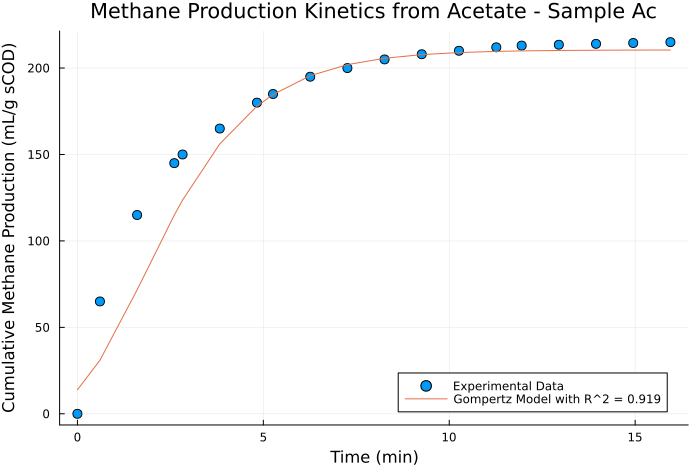
\includegraphics[width=.9\linewidth]{../plots/BMPs/Acetate/methane_kinetics_acet_test_ac.png}
\end{center}

\begin{center}
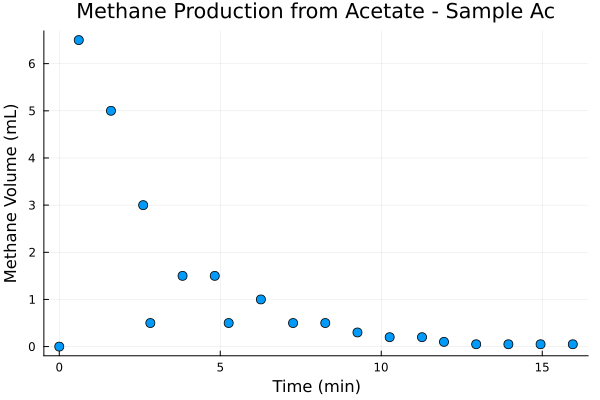
\includegraphics[width=.9\linewidth]{../plots/BMPs/Acetate/acet_test_ac_min.png}
\end{center}

\subsection{Acetate Test 4}
\label{sec:org047337c}
Το section αυτό αναφέρεται στη δοκιμή με 100 μL οξικό στο δείγμα (4).

\textbf{acet\textsubscript{test}\textsubscript{4}}
\begin{minted}[breaklines=true,breakanywhere=true]{julia}

### Data Analysis on Sample 4 ###

<<date_saving_acetate>>

inds = 41:50
exp_meth_vol = [0, 4, 10, 9, 4, 5, 5, 4, 3, 3]
exp_name = "acet_test_4"
source = "Acetate"
sample = "Sample 4"
input_cod = 0.1

<<bmp_data_processing>>
<<bmp_curve_fitting>>
model_acet_4 = vcat(sample, model_params, r_squared)
<<bmp_data_plotting>>
\end{minted}

\begin{table}[htbp]
\caption{Κινητικά δεδομένα}
\centering
\begin{tabular}{lrrrr}
Timestamp & Seconds & Minutes & Methane\textsubscript{Volume} & Cumulative\textsubscript{Methane}\textsubscript{Volume}\\[0pt]
\hline
29/03\textsubscript{12}:29 & 0.0 & 0.0 & 0 & 0\\[0pt]
29/03\textsubscript{12}:29 & 13.397 & 0.2233 & 4 & 4\\[0pt]
29/03\textsubscript{12}:30 & 73.405 & 1.2234 & 10 & 14\\[0pt]
29/03\textsubscript{12}:31 & 133.4 & 2.2233 & 9 & 23\\[0pt]
29/03\textsubscript{12}:32 & 159.347 & 2.6558 & 4 & 27\\[0pt]
29/03\textsubscript{12}:33 & 219.346 & 3.6557 & 5 & 32\\[0pt]
29/03\textsubscript{12}:34 & 279.335 & 4.6556 & 5 & 37\\[0pt]
29/03\textsubscript{12}:35 & 339.339 & 5.6556 & 4 & 41\\[0pt]
29/03\textsubscript{12}:36 & 399.338 & 6.6556 & 3 & 44\\[0pt]
29/03\textsubscript{12}:37 & 459.361 & 7.6560 & 3 & 47\\[0pt]
\end{tabular}
\end{table}

\begin{center}
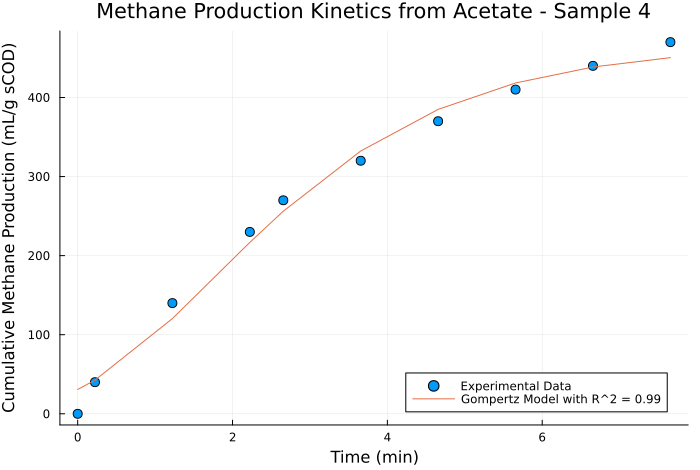
\includegraphics[width=.9\linewidth]{../plots/BMPs/Acetate/methane_kinetics_acet_test_4.png}
\end{center}

\begin{center}
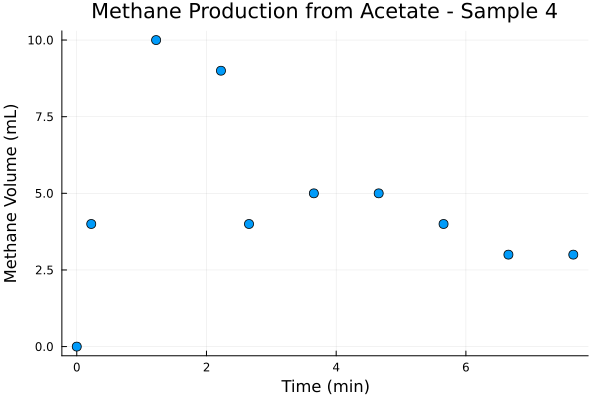
\includegraphics[width=.9\linewidth]{../plots/BMPs/Acetate/acet_test_4_min.png}
\end{center}

\subsection{Acetate Test 2}
\label{sec:org3099e1f}
Το section αυτό αναφέρεται στη δοκιμή με 100 μL οξικό στο δείγμα (2).

\textbf{acet\textsubscript{test}\textsubscript{2}}
\begin{minted}[breaklines=true,breakanywhere=true]{julia}

### Data Analysis on Sample 2 ###

<<date_saving_acetate>>

inds = 44:57
exp_meth_vol = [0, 4, 7, 5.5, 4.5, 2.5, 2, 1, 1, 1, 0.5, 0.5, 0.45, 0.05]
exp_name = "acet_test_2"
source = "Acetate"
sample = "Sample 2"
input_cod = 0.1

<<bmp_data_processing>>
<<bmp_curve_fitting>>
model_acet_2 = vcat(sample, model_params, r_squared)
<<bmp_data_plotting>>
\end{minted}

\begin{table}[htbp]
\caption{Κινητικά Δεδομένα}
\centering
\begin{tabular}{lrrrr}
Timestamp & Seconds & Minutes & Methane\textsubscript{Volume} & Cumulative\textsubscript{Methane}\textsubscript{Volume}\\[0pt]
\hline
29/03\textsubscript{12}:31 & 0.0 & 0.0 & 0.0 & 0.0\\[0pt]
29/03\textsubscript{12}:32 & 25.947 & 0.4324 & 4.0 & 4.0\\[0pt]
29/03\textsubscript{12}:33 & 85.946 & 1.4324 & 7.0 & 11.0\\[0pt]
29/03\textsubscript{12}:34 & 145.935 & 2.4322 & 5.5 & 16.5\\[0pt]
29/03\textsubscript{12}:35 & 205.939 & 3.4323 & 4.5 & 21.0\\[0pt]
29/03\textsubscript{12}:36 & 265.938 & 4.4323 & 2.5 & 23.5\\[0pt]
29/03\textsubscript{12}:37 & 325.961 & 5.4327 & 2.0 & 25.5\\[0pt]
29/03\textsubscript{12}:38 & 386.204 & 6.4367 & 1.0 & 26.5\\[0pt]
29/03\textsubscript{12}:38 & 427.148 & 7.1191 & 1.0 & 27.5\\[0pt]
29/03\textsubscript{12}:39 & 487.142 & 8.1190 & 1.0 & 28.5\\[0pt]
29/03\textsubscript{12}:40 & 547.153 & 9.1192 & 0.5 & 29.0\\[0pt]
29/03\textsubscript{12}:41 & 607.15 & 10.1192 & 0.5 & 29.5\\[0pt]
29/03\textsubscript{12}:42 & 667.16 & 11.1193 & 0.45 & 29.95\\[0pt]
29/03\textsubscript{12}:43 & 722.272 & 12.0379 & 0.05 & 30.0\\[0pt]
\end{tabular}
\end{table}

\begin{center}
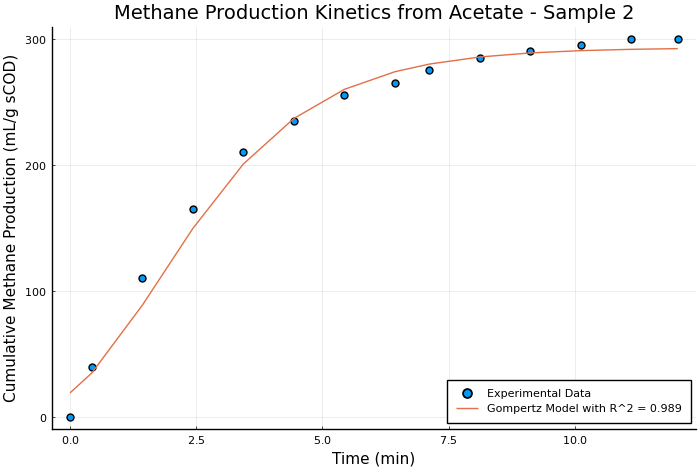
\includegraphics[width=.9\linewidth]{../plots/BMPs/Acetate/methane_kinetics_acet_test_2.png}
\end{center}

\begin{center}
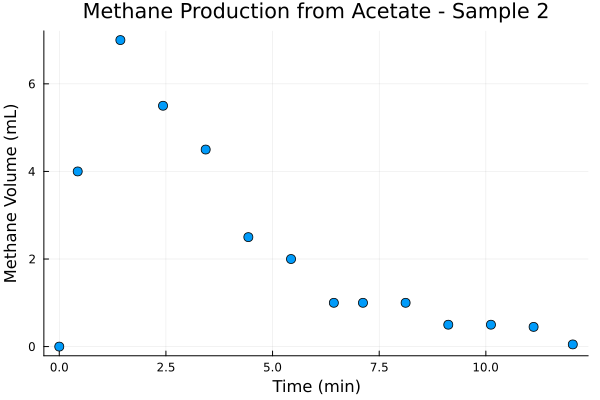
\includegraphics[width=.9\linewidth]{../plots/BMPs/Acetate/acet_test_2_min.png}
\end{center}

\subsection{Παραγωγή μεθανίου χωρίς feed από το δείγμα Ac}
\label{sec:org5159c66}
Όπως προαναφέρθηκε, το δείγμα Ac παρήγαγε μεθάνιο χωρίς να τροφοδοτηθεί με κάτι για κάποιον ανεξήγητο λόγο. Καθώς έχουμε πειραματικά δεδομένα για αυτή την κατανάλωση (και μάλιστα 2 data sets), θα γίνει και μία ανάλυση για αυτό.

\textbf{no\textsubscript{feed}\textsubscript{ac}\textsubscript{1}}
\begin{minted}[breaklines=true,breakanywhere=true]{julia}

### No Feed Data Analysis ###

<<date_saving_acetate>>

inds = 1:17
exp_meth_vol = [0, 9, 3, 2, 3, 3, 3, 2.5, 2.5, 2.5, 1.5, 3, 1, 1, 1.5, 0.5, 0.1]
exp_name = "no_feed_ac_1"
source = "No_Feed"
sample = "Sample Ac"
kinetics = false

<<bmp_data_processing>>
<<bmp_data_plotting>>
\end{minted}

\textbf{no\textsubscript{feed}\textsubscript{ac}\textsubscript{2}}
\begin{minted}[breaklines=true,breakanywhere=true]{julia}

<<date_saving_acetate>>

inds = 18:33
exp_meth_vol = [0, 3, 2, 2, 2, 3, 2, 2, 3, 2, 2.5, 2.5, 2, 2.5, 2.5, 2]
exp_name = "no_feed_ac_2"
source = "No_Feed"
sample = "Sample Ac"
kinetics = false

<<bmp_data_processing>>
<<bmp_data_plotting>>
\end{minted}

\subsection{Update all helper}
\label{sec:org90fc6c1}
Σε αυτό το section θα υπάρχει ένα helper code block που θα κάνει evaluate όλα τα παραπάνω. Έτσι, αν αλλάξει κάτι το οποίο επηρεάζει περισσότερα από ένα code blocks, θα μπορούν να γίνουν updated ταυτόχρονα πιο εύκολα. Επίσης, μία επιπλέον χρησιμότητα του code block αυτού είναι ότι αποθηκεύει ένα CSV που συγκεντρώνει όλα τα δεδομένα των κινητικών παραμέτρων από την προσαρμογή που έγινε παραπάνω, το οποίο είναι χρήσιμο για συγκρίσεις, παρόλο που τα συγκεκριμένα πειράματα δεν είναι τόσο σημαντικό να συγκριθούν.

\textbf{update\textsubscript{acetate}\textsubscript{tests}}
\begin{minted}[breaklines=true,breakanywhere=true]{julia}

<<acet_test_0>>
<<acet_test_1>>
<<acet_test_2>>
<<acet_test_4>>
<<acet_test_ac>>
<<no_feed_ac_1>>
<<no_feed_ac_2>>

model_fit_table = Tables.table(vcat(reshape(model_acet_ac, 1, 5), reshape(model_acet_0, 1, 5), reshape(model_acet_1, 1, 5), reshape(model_acet_2, 1, 5), reshape(model_acet_4, 1, 5)), header = [:Sample_Name, :Methane_Production_Potential, :Methane_Production_Rate, :Lag_Time, :R_squared])
CSV.write(datadir("exp_pro", "methane_from_acetate_kinetics.csv"), model_fit_table)
DataFrame(model_fit_table)

\end{minted}

\subsection{Γενικά σχόλια για αυτόν τον κύκλο πειραμάτων}
\label{sec:org985391b}
Ο πρώτος αυτός κύκλος πειραμάτων ήταν για την δοκιμή προσθήκης οξικού οξέος, του ιδανικού υποστρώματος της μεθανογένεσης, για να δούμε πως θα αντιδράσει σε αυτό το σύστημα. Δεν έχει τόσο συγκριτικό χαρακτήρα μεταξύ των πειραμάτων (παρόλο που ένα σχόλιο που μπορεί να γίνει είναι πως τα πειράματα τα οποία ήταν ίδια πρακτικά στην αρχή, είχαν αρκετά διαφορετική απόκριση στην προσθήκη οξικού), αλλά τον χαρακτήρα της βέλτιστης δυνατής μεθανογένεσης από κάποιο υπόστρωμα. Από την μελέτη αυτή, προέκυψαν αρκετά συμπεράσματα.

Ένα ενδιαφέρον σχόλιο είναι πως το σύστημα ανταποκρίνεται στην προσθήκη του οξικού πολύ γρήγορα (μετά από μερικά δευτερόλεπτα κιόλας βλέπουμε παραγωγή μεθανίου) και στο μοντέλο αυτό μεταφράζεται ως μηδενικό lag-phase.

Το δείγμα 4 είχε αναπάντεχα υψηλό ρυθμό παραγωγής μεθανίου, το οποίο φάνηκε από το γεγονός ότι παράχθηκε την μέγιστη ποσότητα οξικού που περιμέναμε σε περίπου 7 λεπτά ενώ τα υπόλοιπα χρειάστηκαν τουλάχιστον 15 λεπτά. Αυτό φάνηκε και στο μοντέλο, όπου το δείγμα αυτό είχε πολύ υψηλό ειδικό ρυθμό παραγωγής μεθανίου. Το δείγμα Ac ήταν αυτό που παρήγαγε αέριο χωρίς κάποιο υπόστρωμα. Μόλις προστέθηκε οξικό, αντέδρασε σε αυτό και ο ρυθμός του αυξήθηκε, αλλά επιβράδυνε πολύ γρήγορα, με αποτέλεσμα να έχει πολύ αργό ρυθμό παραγωγής μεθανίο και το χαμηλότερο δυναμικό παραγωγής μεθανίου. Μπορεί η αλλαγή αυτή να ευθύνεται σε αυτήν την απόκριση. Τα δείγματα 0 και 4 είχαν πολύ μεγαλύτερη παραγωγικότητα από τα άλλα 3, χωρίς να υπάρχει κάποια εύκολη εξήγηση για αυτό.
\end{document}
